\section*{Collections}
	Collections sind Datenstrukturen für Gruppen von Elementen und fordern einen Import aus dem Packet java.util
	\subsection*{List}
	\begin{minipage}[t]{11cm}
			Eine Liste ist eine Folge von Elementen und kann wie folgt definiert werden:
			\lstinputlisting{code/ArrayList_definition.java}
	\end{minipage}
	\hspace*{0.5cm}
	\begin{minipage}[t]{7.3cm}
		\vspace*{-0.18cm}
		\paragraph*{Iteration mit Enhanced for}
			Besucht jedes Element in einer Collection:
			\lstinputlisting{code/foreach_example.java}
	\end{minipage}
	Einige nützliche Operationen mit Listen:
	\lstinputlisting{code/ArrayList_example.java}
	\subsection*{Set}
		Ein Set ist eine Menge von Elementen, in welchem jedes Element genau einmal vorkommt und wird wie folgt verwendent:
		\lstinputlisting{code/Set_example.java}
		
\section*{Map}
		Abbildung Schlüssel $\rightarrow$ Werte
		\lstinputlisting{code/Map_example.java}
		
\section*{Wrapper-Klassen}
	Collections (bzw. alle Generics) nehmen nur Referenzen, welche primitive Datentypen nicht bringen. Um dennoch int's oder double's in Listen zu speichern, gibt es sogenannte Wrapper-Klassen.\\
	\begin{minipage}[t]{10cm}
		\lstinputlisting{code/Wrapper_AutoBoxing.java}
	\end{minipage}
	\hspace*{0.5cm}
	\begin{minipage}[b]{7.3cm}
		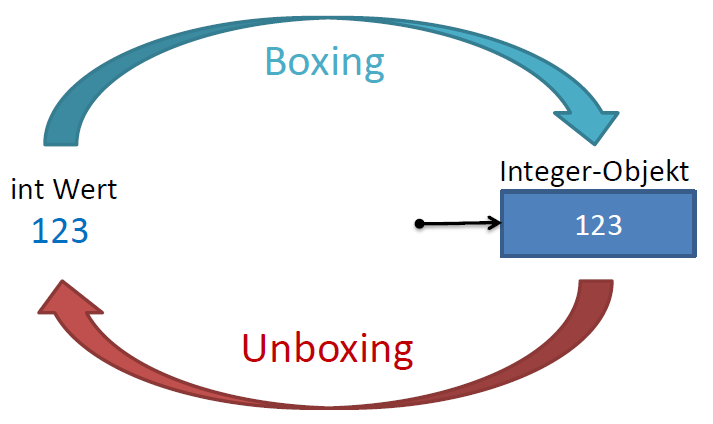
\includegraphics[height=2.5cm, align=t]{pics/boxing_unboxing.PNG}
	\end{minipage}